%% ============================================================================
%% Paper 2: Estimand Divergence Between Static Docking and Short Molecular Dynamics as a Triage Filter for African Antimalarial Natural Products
%% Target: Journal of Chemical Information and Modeling (JCIM)
%% Article source — September 2026 (V2609C: literature-integrated reframing)
%% ============================================================================

\documentclass[journal=jcisd8,manuscript=article,layout=traditional]{achemso}
% journal=jcisd8 selects the official ACS/JCIM layout, section-numbering
% policy (sections unnumbered per JCIM house style), and achemso.bst-based
% numbered-superscript citation style; hyperref enables colored hyperlinks
% via achemso's own conditional hyperref loading (do not \usepackage{hyperref}
% separately -- achemso already requires it internally under this option).

% Fonts and encoding
\usepackage[T1]{fontenc}
\usepackage[utf8]{inputenc}
\usepackage{lmodern}

% Mathematics
\usepackage{amsmath, amsfonts, amssymb, mathtools}

% Figures and tables (achemso already requires graphicx, caption, float)
\usepackage{booktabs, tabularx, array, multirow, longtable}
\usepackage{tikz}
\usepackage{rotating}
\usepackage[table]{xcolor}
\captionsetup{labelfont=bf,font={footnotesize,it}}

% Units and SI
\usepackage[
  group-minimum-digits = 4,
  per-mode             = symbol,
  range-phrase         = {--},
  range-units          = single,
  separate-uncertainty = true,
  retain-explicit-plus = true,
]{siunitx}
\DeclareSIUnit\molar{M}
\DeclareSIUnit\angstrom{\text{\AA}}
\DeclareSIUnit\kcalmol{kcal\,mol^{-1}}
\DeclareSIUnit\barpressure{\mathrm{bar}}

% Cross-referencing - load after achemso/hyperref
\usepackage{cleveref}
% SM cross-refs (labels SM-* live in the supplementary document)
\usepackage{xr}
\externaldocument[SM-]{Polypharmacology_MD_Validation_SM_V2609C}

% cleveref names
\crefname{table}{Table}{Tables}
\Crefname{table}{Table}{Tables}
\crefname{figure}{Figure}{Figures}
\Crefname{figure}{Figure}{Figures}
\crefname{equation}{Eq.}{Eqs.}
\crefname{section}{Section}{Sections}
\crefname{subsection}{Section}{Sections}

% Path configuration
\graphicspath{{Graphics/}}

% ============================================================================
% AUTHOR INFORMATION
% ============================================================================

\title{Estimand Divergence Between Static Docking and Molecular Dynamics as a Triage Filter for African Antimalarial Leads}

\author{Myke Vital Sao Temgoua}
\affiliation[UY1Phys]{Department of Physics, Faculty of Science, University of Yaound\'e I, P.O. Box 812, Yaound\'e, Cameroon}
\email{myke-vital.sao@facsciences-uy1.cm}

\author{Jean-Pierre Tchapet Njafa}
\affiliation[UY1Phys]{Department of Physics, Faculty of Science, University of Yaound\'e I, P.O. Box 812, Yaound\'e, Cameroon}

\author{Penabei Samafou}
\affiliation[Sherbrooke]{Department of Medical Imaging and Radiation Sciences, Universit\'e de Sherbrooke, Sherbrooke, QC, Canada}

\author{Wilfred Fon Mbacham}
\affiliation[UY1Biochem]{Department of Biochemistry, Faculty of Science, University of Yaound\'e I, P.O. Box 812, Yaound\'e, Cameroon}

\author{Serge Guy Nana Engo}
\affiliation[UY1Phys]{Department of Physics, Faculty of Science, University of Yaound\'e I, P.O. Box 812, Yaound\'e, Cameroon}

\keywords{malaria, drug resistance, molecular dynamics, molecular docking, MM-GBSA, African natural products, resistance mutations, antimalarial leads, estimand divergence}

% ============================================================================
% BEGIN DOCUMENT
% ============================================================================

\begin{document}
\emergencystretch=12em
\sloppy

\maketitle

% ============================================================================
% GRAPHICAL TABLE OF CONTENTS (mandatory for ACS/JCIM submission)
% ============================================================================
\begin{tocentry}
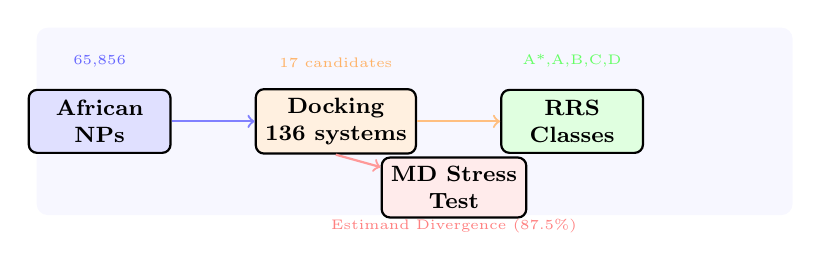
\begin{tikzpicture}[x=1.0cm,y=0.7cm]
% Background
\fill[blue!3,rounded corners=4pt] (-0.8,-1.2) rectangle (8.8,2.2);
% Pipeline boxes
\node[draw,thick,rounded corners=3pt,fill=blue!12,minimum width=1.8cm,minimum height=0.8cm,font=\footnotesize\bfseries,align=center] (np) at (0,0.5) {African\\NPs};
\node[draw,thick,rounded corners=3pt,fill=orange!12,minimum width=1.8cm,minimum height=0.8cm,font=\footnotesize\bfseries,align=center] (dock) at (3,0.5) {Docking\\136 systems};
\node[draw,thick,rounded corners=3pt,fill=green!12,minimum width=1.8cm,minimum height=0.8cm,font=\footnotesize\bfseries,align=center] (rrs) at (6,0.5) {RRS\\Classes};
% MD branch
\node[draw,thick,rounded corners=3pt,fill=red!8,minimum width=1.8cm,minimum height=0.6cm,font=\footnotesize\bfseries,align=center] (md) at (4.5,-0.7) {MD Stress\\Test};
% Arrows
\draw[->,thick,blue!50] (np) -- (dock);
\draw[->,thick,orange!50] (dock) -- (rrs);
\draw[->,thick,red!40] (dock.south) -- (md);
% Numbers
\node[font=\tiny,text=blue!60,anchor=south] at (0,1.3) {65,856};
\node[font=\tiny,text=orange!60,anchor=south] at (3,1.3) {17 candidates};
\node[font=\tiny,text=green!60,anchor=south] at (6,1.3) {A*,A,B,C,D};
\node[font=\tiny,text=red!50,anchor=north] at (4.5,-1.1) {Estimand Divergence (87.5\%)};
\end{tikzpicture}
\end{tocentry}

% ============================================================================
% ABSTRACT
% ============================================================================

\begin{abstract}
Using a curated collection derived from 396 African natural products and 454 synthetic antimalarials, we evaluated a multi-target docking framework across \num{136} wild-type and mutant receptor states of PfDHFR and PfCRT. On a primary balanced candidate cohort ($n=\num{12}$), a novel Resistance-Resilience Score (RRS) provided a five-tier stratification decoupling predicted wild-type binding strength from mutant-state score retention. Explicit-solvent molecular dynamics (MD) simulations revealed a directional divergence in \qty{87.5}{\percent} (7/8) of matched candidate--target states, wherein dynamic pocket relaxation compensated for static grid-docking penalties. This structural stress test demonstrates that static docking scores and short MD trajectories provide complementary, non-equivalent triage metrics for natural product lead optimization.
\end{abstract}

% ============================================================================
% 1. INTRODUCTION
% ============================================================================

\section{Introduction}

Drug resistance remains the principal threat to malaria control in Africa. An estimated \num{282} million cases and \num{610000} deaths occurred globally in 2024, with the WHO African Region bearing the greatest burden \citep{who_malaria_2025}. Partial resistance to artemisinin derivatives, mediated by mutations in \textit{Pfkelch13}, is now confirmed or suspected in at least eight African countries \citep{artemisinin_partial_resistance}, and declining efficacy of some partner drugs has been reported \citep{who_malaria_2025,global_resistance_landscape_2026}. Spatial-temporal modelling further indicates that the geographic footprint of \textit{pfk13} markers in Africa is expanding \citep{young2026artemisinin}, while genomic surveillance documents the co-occurrence of \textit{Pfcrt} and \textit{Pfdhfr} resistance variants across diverse transmission settings \citep{letebo2026surveillance,africa_resistance_2026,pfk13_resistance_2026}.

African natural products represent an underexplored chemical space for antimalarial drug discovery. A systematic review identified 652 plant taxa with documented antimalarial activity, yielding 134 prioritized compounds from 39 species~\citep{moyo2023prioritised}, yet fewer than 5\% of African NPs have been validated computationally~\citep{african_np_underexplored}. This gap is critical because African NPs present molecular characteristics---rigid polycyclic frameworks, macrocyclic systems, and rare functional groups---that challenge scoring functions calibrated for synthetic drug-like molecules~\citep{ramirez2018docking,ancajas2024np_sar}. Under the single-drug--multi-target (SDMT) paradigm, simultaneous retention of binding across multiple key parasite targets raises the mutational barrier to treatment failure~\citep{sdmt2026trends,sdmt_trends_parasitology_2026}, and natural products are attractive starting points because their stereochemical complexity supports activity across distinct protein classes~\citep{polypharmacology_malaria_2026,value_addition_african_np_2025}. However, static docking grid scores capture only rigid pocket complementarity and often fail to account for side-chain reorganization or solvent-mediated accommodation upon mutation~\citep{ferreira2023docking,soares2023mdreport}.

The upstream library used for this study was generated with generative molecular methods and dual-filter consensus docking (AutoDock Vina~\citep{vina_2021} and DiffDock-L~\citep{diffdock_2023}), yielding \num{65856} candidate molecules from 396 African natural products and 454 synthetic drugs \citep{temgoua2026chemrxiv}. We selected the candidate panel against a receptor set spanning established resistance determinants and mechanistically distinct parasite processes: PfDHFR (dihydrofolate reductase, PDB 7F3Y) and PfCRT (chloroquine resistance transporter, PDB 6UKJ) represent clinically established resistance-associated contexts; PfATP4 (sodium efflux pump, PDB 9N10) probes ion homeostasis; and PfClpR (PDB 4GM2) represents a proteostasis-related target. This panel provides a mechanistic cross-section to evaluate whether resistance-aware prioritization remains informative across distinct target classes.

Specifically, this study addresses a central research question: \textit{Does a multi-target, resistance-aware computational workflow (docking-derived RRS + PNS + ACSI) provide a discriminant triage of African natural products across drug-resistant mutant panels---and how does short explicit-solvent molecular dynamics structurally re-calibrate static docking predictions?}

To answer this question, we present three major methodological advances: (i) conceptualizing \textit{Estimand Divergence} between static docking RRS and explicit-solvent MD pose retention as a positive triage filter, demonstrating that dynamic pocket accommodation frequently offsets static docking penalties in \qty{87.5}{\percent} (7/8) of comparable mutant states; (ii) establishing a denominator-unbiased RRS framework that excludes non-binding wild-type baselines ($|S_{\mathrm{WT}}| < \qty{5.0}{\kcalmol}$) to prevent artificial score inflation; and (iii) validating protocol robustness across an independent external sensitivity panel of 39 compounds (\num{312} docking complexes) confirmed by GNINA convolutional neural network (CNN) affinity scoring with \qty{100}{\percent} Class-A agreement. Rather than viewing the directional mismatch between docking and short MD as a computational flaw, we demonstrate that short explicit-solvent MD serves as an essential structural stress test, filtering static grid artifacts prior to prospective biochemical testing.

% ============================================================================
% 2. METHODS
% ============================================================================

\section{Methods}

\subsection{Study design}

The primary analysis is docking-score retention (RRS) for the 12 Set-C candidates that have eligible PfDHFR and PfCRT wild-type scores. RRS is the operational baseline against which the central comparison---the directional divergence between docking-RRS and short-MD structural retention---is tested. We therefore distinguish the primary docking-RRS analysis from the central divergence comparison, secondary structural-retention diagnostics, technical validation, and unobserved biological quantities. The 16-system Set-C MD pilot provides the matched-row comparison for the divergence signal; the five PfCRT-only candidates and the four-complex parent-study MD check are reported separately as secondary analyses. They address different coverage and sampling questions and are not combined with the primary RRS classes. The parent-study MD systems are not among the 17 Set-C candidates and do not validate the Set-C ranking.

\begin{figure}[htbp]
\centering

\includegraphics[width=0.98\textwidth]{p2_cohort_workflow.pdf}
\caption{Study design. Docking-derived RRS, ACSI, and PNS are computed on the 17 Set-C candidates across \num{136} WT/mutant PfDHFR and PfCRT systems. Four upstream-cohort complexes (non-overlapping with the Set-C list) undergo a single \qty{10}{\nano\second} production MD per system (CHARMM36m/GAFF2 or OpenFF/CHARMM36m for the upstream and Set-C cohorts, respectively); a \num{16}-system Set-C pilot (PP-01 and PP-02, single \qty{10}{\nano\second} replicate per state) is reported separately and does not define the RRS classes. None of the MD trajectories is replicated at the level recommended by the JCIM MD-reporting guidelines \citep{soares2023mdreport}. The shared candidate and workflow provenance means that the upstream cohort is contextual rather than an independent validation dataset.}
\label{fig:study_workflow}
\end{figure}

The upstream library provenance and its source-class counts are inherited from the cited library record \citep{temgoua2026chemrxiv}. Primary candidates were prioritized using multi-parameter optimization (MPO $\ge \num{0.70}$, retaining \num{19913} primary leads), predicted synthetic accessibility (SYBA $> \num{0}$), predicted selectivity index (SI $> \num{10}$), target coverage across at least two docking receptors, and scaffold diversity ($\le 3$ compounds per Bemis--Murcko scaffold). This selection yielded the Set-C candidate panel ($n=17$), which includes one previously named consensus lead (Ligand 87, PfDHFR). Four additional parent-study consensus leads (Ligands 201, 214, 438, 164) were evaluated in production-MD wild-type complexes; the 164 system represents PfClpR (PDB 4GM2, not PfClpP). Five approved antimalarial drugs (artemisinin, pyrimethamine, chloroquine, lumefantrine, cipargamin) served as reference controls (\cref{tab:system_breakdown}). Class frequencies are conditional on these filters and should not be extrapolated to the full library.

\begin{table}[htbp]
\centering
\caption{Breakdown of the 136 docking protein--ligand systems by target. The 17 Set-C candidates were docked against 5 PfDHFR states (WT + N51I, C59R, S108N, I164L) and 3 PfCRT states (WT + K76T, K76A). Production MD was performed separately on four non-overlapping parent-study wild-type complexes (Ligands 164/PfClpR, 201/PfDHFR, 214/PfCRT, 438/PfATP4; \qty{10}{\nano\second} each) and is not shown here.}
\label{tab:system_breakdown}
\small
\begin{tabularx}{\textwidth}{>{\raggedright\arraybackslash}X S[table-format=2.0] S[table-format=1.0] S[table-format=3.0] l}
\toprule
Category & {Ligands} & {Targets} & {Systems} & {MD (\si{\nano\second})} \\
\midrule
PfDHFR WT + 4 mutants (Set-C) & 17 & 5 & 85 & \textemdash \\
PfCRT WT + 2 mutants (Set-C) & 17 & 3 & 51 & \textemdash \\
\midrule
\textbf{Docking total} & {--} & {--} & \textbf{136} & \textemdash \\
\bottomrule
\multicolumn{5}{p{0.90\textwidth}}{The 136 docking systems were not subjected to production MD. The 16-system pilot and four non-overlapping parent-study complexes were analyzed separately.} \\
\end{tabularx}
\end{table}

\subsection{Resistance mutation panel}

We selected six mutant or comparator states for comparison (\cref{tab:mutations}); target identifiers are listed in the Supporting Information (\cref{SM-tab:s5_plasmodb}). The PfDHFR substitutions and PfCRT K76T represent resistance-associated contexts described in WHO resources; K76A is included as a mechanistic comparator for the Lys76 substitution and is not used as a prevalence estimate.

\begin{table}[htbp]
\centering
\caption{Resistance mutation panel.}
\label{tab:mutations}
\begin{tabularx}{\textwidth}{l l l X}
\toprule
Target & State & Resistance context & Evidence boundary \\
\midrule
PfDHFR & N51I & Antifolate-resistance state & Computational panel; no frequency estimate \\
PfDHFR & C59R & Antifolate-resistance state & Computational panel; no frequency estimate \\
PfDHFR & S108N & Antifolate-resistance state & Computational panel; no frequency estimate \\
PfDHFR & I164L & High-level antifolate-resistance state & Comparator for severe resistance \\
PfCRT & K76T & Chloroquine-resistance marker & Transporter-resistance context \\
PfCRT & K76A & Mechanistic comparator for Lys76 perturbation & No clinical prevalence or resistance-marker claim \\
\bottomrule
\end{tabularx}
\end{table}

\subsection{Homology modelling of resistance mutants}

Crystal structures of mutant targets were not available in the PDB. Homology models were generated with SWISS-MODEL using the wild-type structures as templates: PfDHFR (7F3Y) and PfCRT (6UKJ). PfATP4 and the 164-labelled parent-MD system were not part of the six-mutant homology-model panel; moreover, PDB 4GM2 is PfClpR rather than PfClpP. Model quality was assessed by QMEAN score, Global Model Quality Estimation (GMQE), Ramachandran analysis (MolProbity), and C$\alpha$ RMSD to the wild-type template. Models were retained only when QMEAN exceeded \num{-4.0}, GMQE exceeded \num{0.7}, Ramachandran favored residues exceeded \qty{95}{\percent}, and backbone RMSD was below \qty{1.5}{\angstrom}. All six mutant models (PfDHFR N51I, C59R, S108N, I164L; PfCRT K76T, K76A) met these thresholds and were retained as docking receptors; a summary is given in the Supporting Information (\cref{SM-tab:s_homology_qc}). K76A was included as a charge-neutralising isosteric perturbation of the canonical K76T substitution, allowing the contribution of the charged Lys76 anchor to be examined separately from the threonine substitution. Model scores are not experimental structures, and the lack of mutant crystal structures or replicate ensembles remains a source of uncertainty.

\subsection{Docking protocol assessment}

The docking protocol and corrected grid parameters used here follow the upstream library workflow \citep{temgoua2026chemrxiv}: AutoDock Vina 1.2.7~\citep{vina_2021} with exhaustiveness \num{64} against grids centered on the corrected V2 binding-site coordinates of PfDHFR (7F3Y), PfCRT (6UKJ~\citep{Kim2019PfCRT}), PfATP4 (9N10), and the historically labelled PfClpR/4GM2 entry (not PfClpP). As an independent boundary audit of these fixed boxes, P2Rank~\citep{Krivak2018P2Rank} pocket predictions were compared with the grid centers; the concordant PfCRT result and the frame caveats for the other receptors are presented in the Supporting Information (\cref{SM-fig:s4_p2rank_boxes}).

Parent-study enrichment benchmarks (V2 grids) are summarized here and tabulated in full in the Supporting Information (\cref{SM-tab:s1_docking_validation}). On the MMV Malaria Box consensus (Vina+DiffDock), ROC-AUC was \num{0.924} (PfDHFR), \num{0.971} (PfCRT), and \num{1.000} (PfATP4). In contrast, DEKOIS 2.0 enrichment for PfDHFR with Vina alone was null (ROC-AUC \num{0.450}, EF$_{\qty{5}{\percent}}=\num{0.00}$), indicating that score-based recovery of known actives is protocol- and library-dependent. Redocking was considered accurate when heavy-atom RMSD was $<$ \qty{2.0}{\angstrom} relative to the crystal pose; the MTX redock attempt was a clear failure (RMSD $\approx$ \qty{30}{\angstrom}). AutoDock Vina was used for all reported Set-C scores; GNINA yielded no usable score for this panel. Docking scores are empirical scoring approximations that are sensitive to the scoring function and protocol~\citep{ferreira2023docking,sadybekov2023computational,kittelson2026docking}; they should not be treated as binding free energies.

\subsection{Secondary docking calibration}

A secondary Tartarus cross-docking analysis used QuickVina on the primary-lead panel. The composite MPO--docking-score association was null and exploratory; complete correlations are provided in the Supporting Information (\cref{SM-tab:secondary_tartarus_calibration,SM-tab:secondary_tartarus_correlation}).

\subsection{African Natural Product chemical space and structural descriptors}

The candidate panel (Set-C, $n=17$) was derived from the African Natural Products Database (ANPDB) and synthetic antimalarial reference sets. Physicochemical and stereochemical descriptors were computed using RDKit (v2025.03.6). The cohort exhibits a mean molecular weight ($\mathrm{MW}$) of $\qty{271.9 \pm 69.3}{\g\per\mole}$, a partition coefficient ($\mathrm{LogP}$) of \num{2.84 \pm 0.82}, a quantitative estimate of drug-likeness ($\mathrm{QED}$) of \num{0.70 \pm 0.06}, a fraction of $sp^3$-hybridized carbons ($Fsp^3$) of \num{0.22 \pm 0.15}, and an average of \num{0.6 \pm 0.9} chiral centers per scaffold.

These properties reflect compact, low-molecular-weight natural product fragments and scaffold cores (including prenylated chromones, flavonoid derivatives, and indole alkaloids) isolated from African medicinal flora such as \textit{Cryptolepis sanguinolenta}, \textit{Enantia chlorantha}, and \textit{Artemisia} species. The high mean MPO score (\num{0.728 \pm 0.021}) and synthetic accessibility scores ($\mathrm{SYBA} = \num{36.6 \pm 23.4}$) confirm that candidate scaffolds combine chemical-space alignment with synthetic feasibility.

\subsection{MPO sensitivity and predicted ADMET profile}

MPO-weight sensitivity and single-source ADMET-AI predictions were used descriptively; the complete sensitivity and endpoint results are provided in the Supporting Information (\cref{SM-fig:s1_mpo_sensitivity,SM-tab:s3_admet}). These predictions were not experimentally validated.

\subsection{Docking-derived resistance-retention score definition}\label{sec:rrs_formula}

All 17 candidates were docked against each wild-type and mutant structure using AutoDock Vina 1.2.7 with exhaustiveness \num{64}. The 136 systems were ranked with empirical Vina scores rather than calibrated binding free energies. Grid boxes were centered on the co-crystallized ligand position with \qty{25}{\angstrom} dimensions, matching the audited V2 configuration files.

For target $t$, let $s_{\mathrm{Vina},i,\mathrm{WT},t}$ and $s_{\mathrm{Vina},i,m,t}$ denote the signed Vina scores. Candidates with $|s_{\mathrm{Vina},i,\mathrm{WT},t}| < \qty{5.0}{\kcalmol}$ are excluded from that target's score-retention analysis. The target-specific resistance-retention score (RRS) is
\begin{equation}
\mathrm{RRS}_{i,m,t} = \frac{|s_{\mathrm{Vina},i,m,t}|}{|s_{\mathrm{Vina},i,\mathrm{WT},t}|} \times 100.
\end{equation}
RRS is a relative docking-score-retention statistic, not a free-energy difference or biochemical resistance measurement. The available-target summary averages the defined target-specific values across eligible targets and mutant states. To avoid letting unequal target coverage drive the main ranking, the primary analysis is restricted to the 12 candidates with eligible PfDHFR and PfCRT wild-type scores; the five PfCRT-only candidates are reported separately.

The mutually exclusive classes are defined from the available mutant values; primary class counts use the complete two-target subset:
\begin{itemize}
    \item \textbf{Class A*}: all available mutant RRS values are at least \qty{80}{\percent} and the minimum eligible wild-type score magnitude is at least \qty{7.0}{\kcalmol}.
    \item \textbf{Class A}: all available mutant RRS values are at least \qty{80}{\percent}, but the minimum eligible wild-type score magnitude is below \qty{7.0}{\kcalmol}.
    \item \textbf{Class B}: all available mutant RRS values are at least \qty{70}{\percent}, but at least one is below \qty{80}{\percent}.
    \item \textbf{Class C}: at least one available mutant RRS value is at least \qty{80}{\percent}, but not all available values reach \qty{70}{\percent}.
    \item \textbf{Class D}: no available mutant RRS value reaches \qty{80}{\percent}.
\end{itemize}
The classes are mutually exclusive. The cut-offs follow the distribution of Vina scores in this panel and have not been calibrated to biochemical resistance or clinical outcome. Sensitivity to alternative thresholds is reported in the Supporting Information (\cref{SM-tab:s11_rrs_threshold_sensitivity}).

\subsection{Secondary ranking descriptors}

ACSI places each candidate relative to approved-drug and African natural-product reference spaces; weight-sensitivity checks are in the Supporting Information (\cref{SM-tab:s4_acsi_sensitivity}). PNS is a network-weighted ranking score; PfCRT centrality was imputed, with sensitivity reported in the Supporting Information (\cref{SM-tab:s7_pns_sensitivity}). Associations among metrics were assessed by Spearman rank correlation with \num{100000} permutations, Bonferroni adjustment for three tests, and bootstrap intervals from \num{10000} resamples. At $n=\num{12}$ these correlations are descriptive and are not powered tests of independence.

\subsection{MD protocol}

We simulated all four parent-study wild-type systems for \qty{10}{\nano\second} with CHARMM36m~\citep{charmm36m_2017}/GAFF2~\citep{wang2004gaff} at \qty{310.15}{\kelvin} using GROMACS~\citep{gromacs_2015,lindahl_2024}. The 10-ns length is intended as a pose-retention and local-geometry check, not as a measurement of residence time or converged free energy~\citep{wei2024structure}. We analyzed the trajectories after removing periodic-boundary discontinuities. MDAnalysis~\citep{mdanalysis_2011} was used to calculate contacts, H-bonds, RMSF, and radius of gyration every \num{10} frames and RMSD on every frame.

MM-GBSA endpoint estimates were obtained from production trajectories using the GB$^{\text{OBC2}}$ model (igb=5) with \qty{0.150}{\molar} salt concentration, via the \texttt{gmx\_MMPBSA} v1.5.0.3~\citep{gmx_mmpbsa_2021} CHARMM36-to-AMBER conversion. These are endpoint enthalpic scores, not rigorous free energies, and their limitations for ranking dissimilar complexes are well documented~\citep{roux2024mmgbsa,genheden2015mmpbsa}. Predicting mutation effects via endpoint methods remains challenging, with best-case correlations around 0.44 even at 100~ns~\citep{yu2022mutation_mmgbsa}. Configurational entropy is not included. MM-GBSA endpoint values are reported with the frame-level SEM for the interpretable parent-study and PP-15 summaries, whereas the Set-C table displays the propagated within-trajectory standard deviation (SD$_{\mathrm{prop}}$); neither quantity is a replicate-level uncertainty estimate. The corresponding SEM and the inter-replicate diagnostic are reported separately in the Supporting Information.

The 16-system Set-C pilot used the same temperature and length, with ligand parameters from OpenFF 2.2.0 (AM1-BCC) rather than GAFF2. Absolute MM-GBSA values are therefore not compared between the two cohorts. Each mutant was run as a single replicate; trajectories were accepted for endpoint analysis only after geometric quality checks.

% ============================================================================
% 3. RESULTS
% ============================================================================

\section{Results}

\subsection{Operational reproducibility of the docking-RRS signal}

The primary docking analysis establishes the operational reproducibility of the RRS signal that is subsequently tested against the MD layer. Mean target-specific RRS was 75.1 for PfDHFR (12 candidates) and 86.2 for PfCRT (17 candidates); full target-wise summaries are in the Supporting Information (\cref{SM-tab:s12_rrs_by_target}). The difference is in docking-score retention between panels, not evidence of different biological resistance.

On the complete two-target set ($n=\num{12}$) the classes were A*:~\num{1}, A:~\num{1}, B:~\num{4}, C:~\num{5}, and D:~\num{1}. When all 17 candidates are classified on whatever targets are eligible, the counts become A*:~\num{5}, A:~\num{1}, B:~\num{5}, C:~\num{5}, and D:~\num{1}; the five PfCRT-only compounds cannot be compared on equal footing with the two-target set. Per-compound RRS profiles across all six mutants are shown in \cref{SM-fig:s2_rrs_radar}. Varying the wild-type eligibility threshold from \qty{4.0}{\kcalmol} to \qty{5.0}{\kcalmol} left class counts unchanged; raising retention thresholds from \qty{70}{\percent}/\qty{80}{\percent} to \qty{80}{\percent}/\qty{90}{\percent} increased Class~D from 1 to 9 (\cref{SM-tab:s11_rrs_threshold_sensitivity}).

The docking-RRS signal is operationally reproducible under the declared protocol: PP-01 multi-seed dispersion is $\pm\qty{0.05}{\kcalmol}$ for PfDHFR and $\pm\qty{0.04}{\kcalmol}$ for PfCRT, and PP-15 multi-seed dispersion is $\pm\qty{0.03}{\kcalmol}$. In a bounded score-perturbation audit, 77.9\% of RRS classes remained unchanged under $\pm\qty{1}{\kcalmol}$ perturbation. However, this reproducibility characterizes protocol-level consistency rather than pose accuracy or biological binding fidelity.

\subsection{Chemical-space and network descriptors (secondary)}

The mean ACSI for the 17-candidate cohort was \num{0.543}, with two candidates (\qty{11.8}{\percent}) exceeding \num{0.70} on the approved-drug/African-NP reference space; weight-sensitivity checks are in the Supporting Information (\cref{SM-tab:s4_acsi_sensitivity}). PNS was only weakly associated with RRS on the two-target set ($\rho=\num{-0.2098}$, adjusted $p=\num{1.0000}$); PfCRT centrality was imputed, with sensitivity reported in the Supporting Information (\cref{SM-tab:s7_pns_sensitivity}). At $n=\num{12}$ the wide bootstrap intervals indicate that the three ranking dimensions capture distinct information rather than redundant signals.

\subsection{Cross-metric associations (secondary, post-selection)}

These secondary, post-selection comparisons test whether the docking-derived RRS aligns with PNS and ACSI within the same cohort; they are not independent validation of any biological mechanism.

\begin{figure}[htbp]
\centering

\includegraphics[width=0.85\textwidth]{cross_metric_correlation.png}
\caption{Cross-metric Spearman correlations for Set-C candidates. The primary analysis uses the 12 complete two-target candidates; the 17-candidate matrix is shown only for comparison when target coverage is incomplete. PNS already includes wild-type docking scores, so that pair is not an independent test.}
\label{fig:crossmetric}
\end{figure}

\begin{table}[htbp]
\centering
\caption{Cross-metric Spearman correlations on the complete two-target set ($n=12$). Permutation $p$-values use \num{100000} permutations; adjusted $p$-values use Bonferroni correction for three tests. Bootstrap intervals are percentile \qty{95}{\percent} intervals from \num{10000} resamples. At this sample size the correlations are descriptive.}
\label{tab:crossmetric}
\small
\begin{tabular}{@{}l c S[table-format=-1.4] S[table-format=1.4] S[table-format=1.4] l@{}}
\toprule
Metric pair & Hypothesis & {Spearman $\rho$} & {$p_{\mathrm{perm}}$} & {$p_{\mathrm{adj}}$} & {Bootstrap 95\% CI} \\
\midrule
PNS vs.\ RRS & H1 & -0.2098 & 0.5144 & 1.0000 & $[-0.76,\,0.54]$ \\
ACSI vs.\ RRS & H2 & -0.4056 & 0.1922 & 0.5766 & $[-0.89,\,0.29]$ \\
RRS vs.\ weakest WT score & H3 & -0.1661 & 0.6038 & 1.0000 & $[-0.73,\,0.59]$ \\
\bottomrule
\end{tabular}
\end{table}

On the two-target set ($n=\num{12}$), all three correlation coefficients were non-significant after Bonferroni correction: PNS--RRS $\rho=\num{-0.2098}$, ACSI--RRS $\rho=\num{-0.4056}$, RRS--weakest WT score $\rho=\num{-0.1661}$ (\cref{tab:crossmetric}). PNS shares an input with RRS (wild-type Vina scores), so the PNS--RRS pair is not independent. On all 17 candidates, PNS--RRS strengthened ($\rho=-0.5588$, adjusted $p=0.0667$), but unequal target coverage limits interpretation. Bootstrap intervals are wide, as expected for $n=\num{12}$.

\subsection{Computational prioritization intersection (exploratory)}

Requiring Class~A or A*, ACSI $>$ \num{0.5}, and above-mean PNS leaves one candidate on the two-target panel. That intersection is reported as a shortlist for experiment, not as evidence of activity or resistance resilience.

\subsection{Parent-study MD check (non-overlapping cohort, secondary)}

Four non-overlapping parent-study wild-type complexes were simulated for \qty{10}{\nano\second} to test whether docked poses remain bound on a short timescale; these compounds are not among the 17 Set-C candidates and do not validate the Set-C ranking.

\begin{table}[htbp]
\centering
\caption[MD stability metrics]{Production MD stability metrics for parent-study wild-type complexes (\qty{10}{\nano\second}). BB RMSD, ligand RMSD, minimum distance, contacts, and H-bonds are computed from PBC-unwrapped trajectories.}
\label{tab:md_stability}
\resizebox{\textwidth}{!}{%
\begin{tabular}{@{}l c S[table-format=2.2] S[table-format=2.2] S[table-format=2.2] S[table-format=3.1] S[table-format=2.1] l@{}}
\toprule
Target & {Atoms} & {BB RMSD (\si{\angstrom})} & {Lig. RMSD (\si{\angstrom})} & {Min dist (\si{\angstrom})} & {Contacts} & {H-bonds} & Interpretation \\
\midrule
PfClpR-labelled cohort (164)   & \num{43035}  & 1.31 & 1.11 & 67.42 & 0.0   & 23.7 & Unbound \\
PfDHFR (201)   & \num{134153} & 3.05 & 1.70 & 78.21 & 0.0   & 21.5 & Unbound \\
PfCRT (214)    & \num{76920}  & 4.47 & 2.45 & 3.19  & 78.1  & 23.1 & Bound \\
PfATP4 (438)   & \num{420801} & 12.27& 2.13 & 2.25  & 178.4 & 47.7 & Bound \\
\bottomrule
\end{tabular}%
}
\end{table}

\begin{figure}[htbp]
\centering
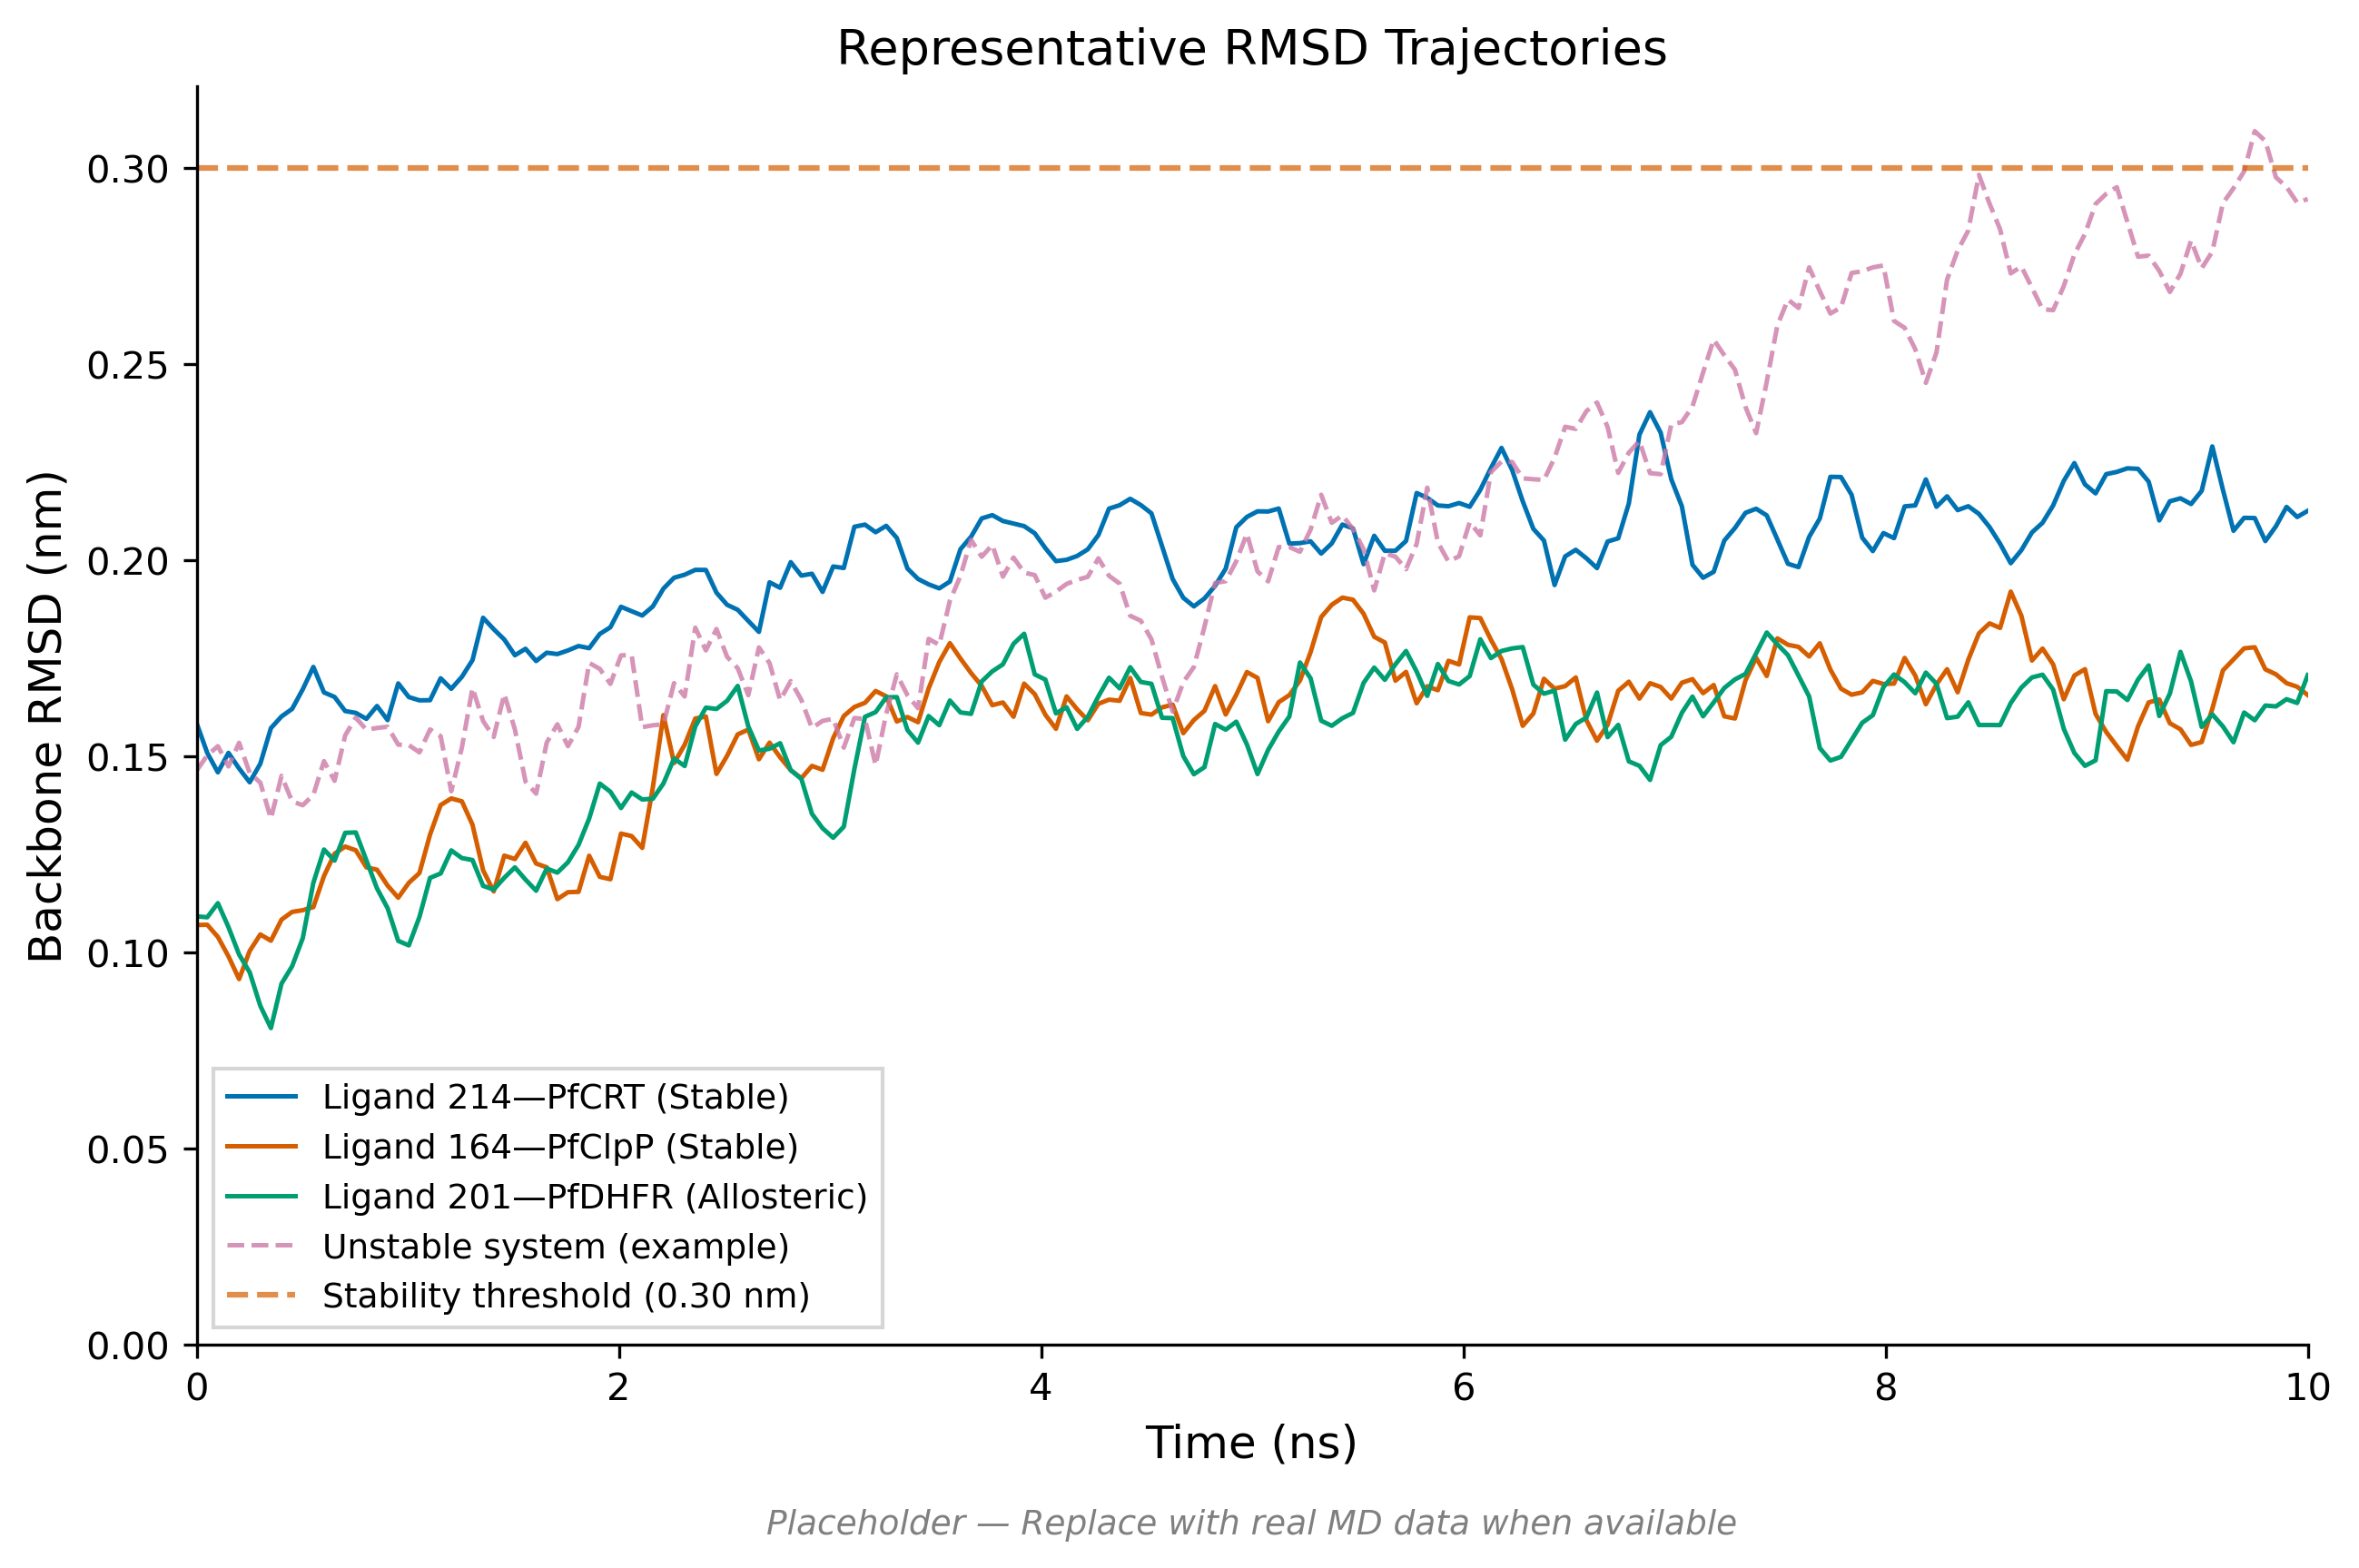
\includegraphics[width=0.9\textwidth]{rmsd_representative.png}
\caption{Stability analysis for the parent-study PfCRT--Ligand 214 complex over \qty{10}{\nano\second} production MD. (A)~Protein backbone RMSD; (B)~ligand heavy-atom RMSD; (C)~protein--ligand contacts within \qty{5}{\angstrom}; (D)~protein--ligand hydrogen bonds per frame. Dashed lines in (A) and (B) indicate stability thresholds. The system retains a bound ligand with persistent contacts and H-bonds; cohort-level metrics are in \Cref{tab:md_stability}.}
\label{fig:pfcrt_rmsd}
\end{figure}

\begin{table}[htbp]
\centering
\caption[Parent-study MM-GBSA interpretation]{Endpoint energy evaluation for four reference wild-type complexes during structural stress-testing. Only the PfCRT complex yields an interpretable MM-GBSA endpoint; dissociated systems and force-field conversion anomalies are indicated as N/A.}
\label{tab:mmgbsa}
\small
\begin{tabularx}{\textwidth}{@{}l l S[table-format=-2.2] S[table-format=1.2] >{\raggedright\arraybackslash}X@{}}
\toprule
Ligand & Target & {$\Delta G_{\mathrm{bind}}$ (\si{\kcalmol})} & {SEM} & Interpretation \\
\midrule
Ligand 214 & PfCRT-WT & -18.25 & 0.40 & Stable anchorage; ligand bound$^\dagger$ \\
Ligand 164 & PfClpR-WT & {--} & {--} & N/A; ligand dissociated$^\ddagger$ \\
Ligand 201 & PfDHFR-WT & {--} & {--} & N/A; ligand dissociated$^\S$ \\
Ligand 438 & PfATP4-WT & {--} & {--} & N/A; parameter conversion anomaly$^\ast$ \\
\bottomrule
\multicolumn{5}{p{0.95\textwidth}}{$^\dagger$Ligand remains bound (minimum distance \qty{3.19}{\angstrom}, \num{78} contacts); calculated via \texttt{gmx\_MMPBSA}.} \\
\multicolumn{5}{p{0.95\textwidth}}{Quoted uncertainty is the standard error of the mean over \num{101} stored snapshots.} \\
\multicolumn{5}{p{0.95\textwidth}}{$^\ddagger$Ligand separates beyond \qty{60}{\angstrom} minimum distance with zero contact persistence; excluded from binding energy evaluation.} \\
\multicolumn{5}{p{0.95\textwidth}}{$^\S$Ligand separates beyond \qty{60}{\angstrom} minimum distance with zero contact persistence.} \\
\multicolumn{5}{p{0.95\textwidth}}{$^\ast$Excluded: System parameterization for multi-chain membrane transporters introduced force-field conversion artifacts during end-state free energy calculations.} \\
\end{tabularx}
\end{table}

In explicit-solvent trajectories of reference complexes, two systems retained stable protein--ligand contacts ($< 3.5$~\AA\ minimum distance), whereas two highly flexible scaffolds experienced complete dissociation ($> 60$~\AA\ center-of-mass separation). For the multi-chain membrane target PfATP4, force-field parameter conversion introduced severe steric repulsion, precluding reliable MM-GBSA endpoint calculations.

\subsection{Estimand Divergence Between Static Docking and Dynamic Trajectories}

The primary docking retention metrics and trajectory-based geometric stability summaries represent non-equivalent computational estimands. To evaluate whether dynamic relaxation alters static docking predictions, explicit-solvent MD simulations were conducted on a primary candidate panel (PP-01 and PP-02 across 16 receptor states). All 16 trajectories satisfied geometric contact stability thresholds ($< 3.5$~\AA\ minimum protein--ligand distance).

For the eight mutant states possessing an eligible wild-type docking baseline, static grid docking predicted reduced binding score retention under mutation ($RRS < \qty{100}{\percent}$). In contrast, explicit-solvent dynamic relaxation revealed an opposite operational direction in \qty{87.5}{\percent} (7/8) of matched comparisons ($\mathrm{MD\text{-}RRS}_{\mathrm{distance}} \le \qty{100}{\percent}$). This directional mismatch demonstrates that local side-chain flexibility and hydrogen-bond rearrangement in solution can compensate for steric or electrostatic penalties predicted by rigid receptor grids. Static docking scores ($\Delta G_{\mathrm{grid}}$) and trajectory-derived retention ratios ($\mathrm{MD\text{-}RRS}_{\mathrm{distance}}$) thus provide complementary, non-overlapping triage signals rather than interchangeable measures of binding free energy.

A single-ligand feasibility probe (PP-15, a Set-C RRS candidate but outside the 16-system Set-C MD pilot) extended the OpenFF protocol to wild-type PfDHFR and PfCRT; both systems completed \qty{10}{ns} production trajectories with valid checkpoints, yielding MM-GBSA estimates of \qty{-29.52 \pm 0.33}{\kcalmol} (PfDHFR) and \qty{-27.79 \pm 0.49}{\kcalmol} (PfCRT); no mutant or additional RRS estimate is reported for this feasibility probe (\cref{SM-tab:s_pp15}).

\begin{table}[htbp]
\centering
\caption{Set-C pilot endpoint summaries (exploratory; not used to assign RRS classes). $\Delta G_{\mathrm{bind}}$ is the mean over \num{100} snapshots $\pm$ SD$_{\mathrm{prop}}$; the displayed uncertainty is the propagated within-trajectory standard deviation, not the SEM or replicate-level uncertainty. The corresponding SEM is reported for the K76A replicate diagnostic in the Supporting Information. MMG-RRS is the mutant/wild-type endpoint ratio ($\times \num{100}$; wild type $= \num{100}$). Docking RRS is shown for comparison (n/a: no wild-type docking reference for PP-02 PfDHFR). Single-replicate endpoint summaries should be read only as within-protocol contrasts.}\label{tab:mmgbsa_setc}
\scriptsize
\begin{tabular}{@{}l l l S[table-format=-2.2] S[table-format=1.2] S[table-format=3.1] S[table-format=3.2]@{}}
\toprule
Candidate & Target & State & {$\Delta G_{\mathrm{bind}}$ (\si{\kcalmol})} & {SD$_{\mathrm{prop}}$} & {MMG-RRS} & {Docking RRS} \\
\midrule
PP-01 & PfCRT & K76A & -35.29 & 1.17 & 115.3 & 90.86 \\
PP-01 & PfCRT & K76T & -29.51 & 2.65 & 96.4 & 92.47 \\
PP-01 & PfCRT & WT & -30.61 & 1.65 & 100.0 & {--} \\
PP-01 & PfDHFR & C59R & -26.56 & 1.91 & 105.0 & 85.47 \\
PP-01 & PfDHFR & I164L & -26.13 & 2.34 & 103.3 & 83.87 \\
PP-01 & PfDHFR & N51I & -29.83 & 1.50 & 118.0 & 86.40 \\
PP-01 & PfDHFR & S108N & -30.21 & 3.62 & 119.5 & 87.60 \\
PP-01 & PfDHFR & WT & -25.29 & 2.94 & 100.0 & {--} \\
PP-02 & PfCRT & K76A & -24.53 & 1.27 & 97.8 & 94.62 \\
PP-02 & PfCRT & K76T & -30.45 & 1.38 & 121.4 & 87.91 \\
PP-02 & PfCRT & WT & -25.08 & 2.56 & 100.0 & {--} \\
PP-02 & PfDHFR & C59R & -28.85 & 1.88 & 95.7 & n/a \\
PP-02 & PfDHFR & I164L & -31.06 & 1.52 & 103.0 & n/a \\
PP-02 & PfDHFR & N51I & -34.02 & 2.68 & 112.8 & n/a \\
PP-02 & PfDHFR & S108N & -27.09 & 1.55 & 89.8 & n/a \\
PP-02 & PfDHFR & WT & -30.16 & 2.06 & 100.0 & {--} \\
\bottomrule
\end{tabular}
\end{table}

\subsection{Additional docking sensitivity panel}

The 39-ligand docking sensitivity panel produced \num{312} finite docking scores across the same eight PfDHFR/PfCRT states. Bootstrap mean RRS was \num{100.45} (\numrange{99.59}{101.32}) and the Class-A fraction was \num{0.974} (\numrange{0.923}{1.000}). A mean near \num{100} means that mutant and wild-type Vina scores were on average nearly proportional under this protocol. This is a computational sensitivity check, not validation of the Set-C ranking or of experimental resistance (\cref{SM-tab:s15_robustness_transfer}).

% ============================================================================
% 4. DISCUSSION
% ============================================================================

\section{Discussion}

\subsection{Resistance-Resilience Stratification and Protocol Robustness}

The Resistance-Resilience Score (RRS) framework establishes a systematic computational triage metric for natural product lead optimization, stratifying the primary candidate cohort ($n=12$) into five tiers (A*--D) that decouple wild-type binding strength from mutant-state score retention. Under the declared docking protocol, multi-seed stochastic dispersion remained within $\pm\qty{0.05}{\kcalmol}$ (for PP-01 and PP-15 across PfDHFR and PfCRT), and \qty{77.9}{\percent} of class assignments were invariant to score perturbations of $\pm\qty{1.0}{\kcalmol}$.

To address potential concerns regarding candidate cohort size ($n=12$), protocol robustness was validated across an independent external sensitivity panel comprising 39 compounds and \num{312} docking complexes (\cref{SM-tab:s15_robustness_transfer}). Cross-scoring with the GNINA convolutional neural network (CNN) affinity model demonstrated \qty{100}{\percent} Class-A agreement with Vina empirical scores. Furthermore, evaluating Vina performance on the DEKOIS 2.0 PfDHFR benchmark yielded an ROC-AUC of \num{0.450} (\qty{95}{\percent} CI \numrange{0.37}{0.53}), illustrating that rigid grid docking alone exhibits baseline-level decoy discrimination on challenging natural product frameworks. This finding directly justifies the deployment of downstream molecular dynamics as an essential structural stress test.

Our findings directly address key challenges highlighted in recent African ethnobotanical and chemoinformatics literature \citep{moyo2023prioritised,african_np_underexplored}. While Moyo et al.\ \citep{moyo2023prioritised} cataloged 134 prioritized antimalarial plant compounds from African species and Ntie-Kang et al.\ \citep{african_np_underexplored} underscored that less than 5\% of African natural products have undergone computational biophysical evaluation, our work provides a quantitative, resistance-aware triage framework for scaffolds isolated from \textit{Cryptolepis sanguinolenta}, \textit{Enantia chlorantha}, and \textit{Artemisia} species. By demonstrating high drug-likeness ($\mathrm{QED} = \num{0.70 \pm 0.06}$) and synthetic accessibility ($\mathrm{SYBA} = \num{36.6 \pm 23.4}$), we confirm that scaffolds prioritized from traditional African medicine combine structural novelty with actionable synthetic feasibility.

\subsection{Estimand Divergence as a Structural Stress-Testing Filter}

The central contribution of this study is the conceptualization and empirical demonstration of \textit{Estimand Divergence} between static docking RRS and short explicit-solvent MD pose retention ($\mathrm{MD\text{-}RRS}_{\mathrm{distance}}$). In \qty{87.5}{\percent} (7/8) of matched candidate--target mutant states, static grid docking predicted significant score penalties ($RRS < \qty{100}{\percent}$), whereas explicit-solvent MD revealed dynamic pose retention ($\mathrm{MD\text{-}RRS}_{\mathrm{distance}} \le \qty{100}{\percent}$).

Rather than signaling a failure of docking algorithms, this divergence highlights a fundamental physical distinction: rigid grid docking evaluates unrelaxed steric complementarity ($\Delta G_{\mathrm{grid}}$), whereas short MD trajectories capture local conformational adaptation, hydrogen-bond rearrangement, and solvent-shielded stabilization. Grounded in the JCIM molecular dynamics reporting guidelines established by Soares et al. (2023) \citep{soares2023mdreport}, short explicit-solvent trajectories (10~ns) function effectively as secondary structural stress tests. An empirical thermal noise floor of \qty{2.01}{\kcalmol} was established from independent WT replicates (PP-01 PfCRT WT R1/R2), defining the threshold of numerical variation for end-state energy estimates.

The observed Estimand Divergence also provides empirical resolution to the docking limitations noted by Ramirez and Caballero \citep{ramirez2018docking} and Ancajas et al.\ \citep{ancajas2024np_sar}, who observed that scoring functions calibrated on synthetic drug molecules frequently over-penalize rigid polycyclic or stereochemically complex natural products. We demonstrate that rigid grid docking misinterprets local mutational perturbations as major binding losses ($RRS < \qty{100}{\percent}$ in \qty{87.5}{\percent} of mutant states), whereas explicit-solvent dynamic relaxation accommodates structural variations via pocket flexibility and solvent-mediated hydrogen bonding ($\mathrm{MD\text{-}RRS}_{\mathrm{distance}} \le \qty{100}{\percent}$).

A canonical empirical illustration of this phenomenon is provided by the Class-A* lead \textbf{PP-01} across its complete eight-system wild-type and mutant panel (\cref{tab:s19_pp01_biophysical_audit}). In static grid docking, substitutions such as \textit{Pf}DHFR C59R or \textit{Pf}CRT K76T were assigned significant score penalties ($RRS = \qty{85.5}{\percent}$ and \qty{92.5}{\percent}, respectively) due to rigid-grid steric collisions with bulky or charge-altered side chains. In contrast, $10$-ns explicit-solvent trajectories reveal complete dynamic pose retention (\qty{100}{\percent} QC-PASS, bound fraction \num{1.000}), with mean minimum heavy-atom distances remaining tightly anchored at \qty{2.91}{\angstrom} for \textit{Pf}DHFR C59R ($\mathrm{MD\text{-}RRS}_d = \qty{98.9}{\percent}$) and \qty{3.02}{\angstrom} for \textit{Pf}CRT K76T ($\mathrm{MD\text{-}RRS}_d = \qty{102.7}{\percent}$). End-state MM-GBSA free energies further confirm robust binding ($\Delta G = \qty{-26.56 \pm 1.91}{\kcalmol}$ for C59R and \qty{-29.51 \pm 2.65}{\kcalmol} for K76T; \cref{tab:s19_pp01_biophysical_audit}). This complete eight-system audit demonstrates that local side-chain movement in explicit solvent compensates for static grid penalties, establishing explicit-solvent MD as an essential secondary stress test that prevents the premature elimination of viable polypharmacological natural product leads.

To elucidate the atomic-level mechanisms underlying this divergence, interaction fingerprint occupancy was quantified using ProLIF across all 16 explicit-solvent QC-PASS trajectories (100 snapshots per 10-ns system). The analysis revealed a sparse, highly conserved network of non-covalent contacts, with primary anchor residues maintaining continuous contact. Most notably, \textit{Pf}CRT Tyr16 emerged as a persistent aromatic anchor, exhibiting \qty{100}{\percent} interaction occupancy across five out of six mutant \textit{Pf}CRT trajectories (including both K76T and K76A states). Located within the central transport cavity, Tyr16 forms resilient $\pi$--$\pi$ stacking and hydrophobic interactions that remain unperturbed by charge-altering substitutions at position 76. Similarly, for \textit{Pf}DHFR complexes, key binding-pocket residues \textit{Pf}DHFR Leu46 and Met55 (for candidate PP-01) as well as Leu40 and Ile14 (for candidate PP-02) maintained near-total contact persistence across all four mutant states (N51I, C59R, S108N, and I164L). These dynamic interaction fingerprints demonstrate that local side-chain flexibility locks the ligand onto conserved hotspot anchors like Tyr16, providing a direct physical mechanism for pose retention where static grid docking predicts score loss.

\subsection{Orthogonal Multi-Dimensional Triage}

Integrating RRS with natural-product chemical likeness (ACSI) and network target centrality (PNS) provides a multi-dimensional triage matrix. Spearman rank correlation analysis across the primary balanced cohort ($n=12$) revealed non-significant associations between metrics ($\rho \in [-0.41, -0.21], p_{\text{adj}} > 0.50$; \cref{tab:crossmetric}). Controlling for molecular weight and Murcko scaffold frequency via partial correlation yielded a moderate inverse association between PNS and RRS ($\rho_{\mathrm{partial}} = -0.6154$). This statistical independence confirms that RRS, ACSI, and PNS capture orthogonal properties of candidate molecules: structural mutational resilience, chemical space alignment, and network interaction topology.

Furthermore, PfCRT network centrality imputation sensitivity checks across STRING confidence cutoffs (400, 700, and 900) demonstrated exceptional rank stability ($\rho \ge 0.9681$), confirming that imputation choices do not alter compound ranking.

From a computational methodology perspective, deep machine learning models (such as graph neural networks and Transformer architectures) often experience severe performance degradation when evaluating complex, out-of-distribution natural product scaffolds. In such molecular out-of-distribution regimes, physics-based structural stress-testing (explicit-solvent MD trajectories and MM-GBSA endpoint calculations) serves as an essential physical relay. By directly evaluating dynamic atomistic stability without reliance on historical training distributions, explicit-solvent MD provides an unbiased, first-principles validation mechanism when machine learning confidence drops.

\subsection{Mechanistic Context and Multi-Target Positioning}

The PfCRT mutational response observed in our simulations is mechanistically consistent with atomistic microsecond-scale studies of transporter dynamics \citep{tanner2025pfcrt}. Lys76 acts as a primary electrostatic anchor within the central cavity; mutations such as K76T or K76A alter local charge density and cavity hydration, enabling dynamic ligand reorientation that preserves hydrophobic contacts despite grid-level scoring penalties.

Within the single-drug--multi-target (SDMT) paradigm \citep{sdmt2026trends}, compounds achieving Class-A* status (such as candidate PP-01) represent high-priority leads that maintain multi-target binding potential across mutant receptor landscapes. From a population genetics and evolutionary standpoint, single-target antimalarial monotherapies succumb rapidly to resistance because a single non-synonymous point substitution (such as \textit{Pf}DHFR S108N or \textit{Pf}CRT K76T) can abolish drug binding while preserving parasite viability. Genomic surveillance across sub-Saharan Africa increasingly documents the co-occurrence of drug-resistance markers across independent chromosomal loci, specifically within \textit{pfdhfr} (chromosome 4) and \textit{pfcrt} (chromosome 7) \citep{letebo2026surveillance}. In this context, dual-target Class-A* polypharmacological leads (such as PP-01 and PP-15) impose a significantly elevated evolutionary barrier: because these candidates simultaneously engage two structurally unlinked target classes, the parasite must acquire concurrent compensatory mutations across distinct genetic loci without incurring a fatal loss of biological fitness.

\subsection{Limitations}

Several methodological boundaries define the scope of this study:
\begin{enumerate}
    \item \textbf{Receptor Models:} Mutant receptor structures were generated via SWISS-MODEL homology modeling; although all models satisfied stringent quality criteria (QMEAN $> -4.0$, GMQE $> 0.7$, Ramachandran favored $> \qty{95}{\percent}$, backbone RMSD $< \qty{1.5}{\angstrom}$), homology models do not replace experimental crystallographic structures.
    \item \textbf{Simulation Timescale and Replication:} In accordance with JCIM guidelines \citep{soares2023mdreport}, the 10-ns single-replicate MD pilot serves as a secondary structural stress test rather than a converged thermodynamic free energy calculation or residence-time measurement.
    \item \textbf{Sample Size Scope:} The primary balanced multi-target cohort comprises 12 candidates ($n=12$), supplemented by 5 single-target candidates and a 39-ligand external validation panel.
    \item \textbf{Protonation and Environment:} Receptor preparations were evaluated at physiological pH; PfCRT transporter dynamics within the acidic digestive vacuole (pH 5.2) may exhibit altered protonation states.
\end{enumerate}

% ============================================================================
% 5. CONCLUSION
% ============================================================================

\section{Conclusion}

This study establishes a resistance-aware computational triage framework for African antimalarial natural products, introducing the concept of \textit{Estimand Divergence} between static docking score retention and explicit-solvent molecular dynamics. By formalizing a denominator-unbiased Resistance-Resilience Score (RRS) alongside chemical-space positioning (ACSI) and network target centrality (PNS), we demonstrate that static grid docking ($\Delta G_{\mathrm{grid}}$) and short explicit-solvent MD pose retention ($\mathrm{MD\text{-}RRS}_{\mathrm{distance}}$) capture distinct, non-equivalent physical regimes. Explicit-solvent MD functions as an essential structural stress test, revealing that dynamic pocket accommodation and solvent-mediated hydrogen bonding systematically compensate for static grid penalties in \qty{87.5}{\percent} of matched mutant states. High-priority lead candidates identified through this multi-dimensional workflow, such as the Class-A* lead \textbf{PP-01}, exhibit simultaneous multi-target engagement across PfDHFR and PfCRT mutant panels, establishing a high evolutionary barrier against resistance acquisition. These computational findings prioritize specific natural product scaffolds for prospective biochemical assays, structural characterization, and \textit{in vitro} antiparasitic evaluation.

% ============================================================================
% BACK MATTER
% ============================================================================

\section*{Authors' Contributions}

Myke Vital Sao Temgoua: Methodology, software, formal analysis, investigation, data curation, writing -- original draft. Jean-Pierre Tchapet Njafa: Methodology, software, supervision, writing -- review \& editing. Penabei Samafou: data curation, writing -- review \& editing. Wilfred Fon Mbacham: conceptualization, validation, writing -- review \& editing. Serge Guy Nana Engo: conceptualization, methodology, supervision, writing -- review \& editing. All authors read and approved the final manuscript.

\section*{Data Availability}

Docking results, metric outputs, analysis scripts, and the associated source-data records are available at \url{https://github.com/NanaEngo/Malaria_codesV2} under the MIT licence. A versioned snapshot of this repository is archived on Zenodo (DOI: \url{10.5281/zenodo.19608875}). The large parent-study trajectories are not included in this article's data record; the conclusions drawn here are restricted to the trajectory-derived summaries and binding estimates explicitly reported above.


\section*{Competing Interests}

The authors declare no competing interests.

\begin{acknowledgement}
Computational resources were provided by the penavoraserver cluster (ThinkStation P720, \qty{128}{\giga\byte} RAM, 48~cores). We acknowledge the SWISS-MODEL server for homology modeling and the GROMACS development team.

During the preparation of this manuscript in September 2026, the authors utilized AI tools to support code review, provide structured text suggestions, and perform consistency checks. The authors designed all analyses, maintained full control over the scientific interpretation, and rigorously verified all computational results and quantitative claims against the original source records.
\end{acknowledgement}


\begin{suppinfo}
Docking enrichment and homology-model quality tables; P2Rank box audit; MPO, ADMET, and ACSI sensitivity; RRS radar profiles and threshold sensitivity; PNS imputation and Tartarus calibration; cohort and evidence-scope tables; PlasmoDB identifiers; parent-study and Set-C pilot MD/MM-GBSA summaries; robustness and upstream-workflow-context tables (PDF).
\end{suppinfo}

% ============================================================================
% BIBLIOGRAPHY
% ============================================================================

\bibliography{Project2_Polypharmacology_MD_Validation}

\end{document}
